\documentclass{beamer}
\usepackage{hyperref}
\usepackage[T1]{fontenc}

% other packages
\usepackage{latexsym,amsmath,xcolor,multicol,booktabs,calligra}
\usepackage{graphicx,pstricks,listings,stackengine}

% dummy text; remove it when working on this template
\usepackage{lipsum}

\author{Runze Ma}
\title{Monash Beamer Theme}
\subtitle{Thesis Proposal Presentation}
\institute{Faculty of Information Technology \\ Monash University}
\date{October 2025}
\usepackage{monash} % Keep your theme file if customized

% ---------- Definitions ----------
\def\cmd#1{\texttt{\color{red}\footnotesize $\backslash$#1}}
\def\env#1{\texttt{\color{blue}\footnotesize #1}}
\definecolor{deepblue}{rgb}{0,0,0.5}
\definecolor{deepred}{rgb}{0.6,0,0}
\definecolor{deepgreen}{rgb}{0,0.5,0}
\definecolor{halfgray}{gray}{0.55}

\lstset{
    basicstyle=\ttfamily\small,
    keywordstyle=\bfseries\color{deepblue},
    emphstyle=\ttfamily\color{deepred},
    stringstyle=\color{deepgreen},
    numbers=left,
    numberstyle=\small\color{halfgray},
    rulesepcolor=\color{red!20!green!20!blue!20},
    frame=shadowbox,
}

\begin{document}

% --------------------------------------
% Title Page
% --------------------------------------
\begin{frame}
    \titlepage
    \begin{figure}[htpb]
        \centering
        
\includegraphics[width=0.2\linewidth]{pic/crest.jpg} % your logo file
    \end{figure}
\end{frame}

\begin{frame}
    \tableofcontents[sectionstyle=show,subsectionstyle=show/shaded/hide,subsubsectionstyle=show/shaded/hide]
\end{frame}

% --------------------------------------
\section{Background}

\begin{frame}{Why Beamer?}
    \begin{itemize}[<+-| alert@+>]
        \item \LaTeX{} is widely used in academia, and many universities have their own Beamer themes.
        \item Please use Xe\LaTeX{} compiler for best results.
        \item Original theme: \url{https://github.com/Kha1edze/MONASH-Beamer-Theme}
    \end{itemize}
\end{frame}

% --------------------------------------
\section{Related Work}

\subsection{Beamer Theme Categories}

\begin{frame}{Beamer Theme Types}
    \begin{itemize}
        \item Default \LaTeX{} themes
        \item University-customized themes
        \item This template was modified from the Tsinghua University Beamer theme.
    \end{itemize}
\end{frame}

% --------------------------------------
\section{Research Content}

\subsection{Theme Enhancements}

\begin{frame}{Differences from THU Beamer Theme}
    \begin{itemize}
        \item Color scheme adjustments
        \item University logo
    \end{itemize}
\end{frame}

\subsection{Why Use Beamer}

\begin{frame}{Why Beamer}
    \begin{itemize}
        \item \LaTeX{} is widely adopted in scientific publishing.
    \end{itemize}
    \begin{table}[h]
        \centering
        \begin{tabular}{c|c}
            Microsoft Word & \LaTeX \\
            \hline
            Word processor & Professional typesetting \\
            Easy to learn & Requires basic syntax \\
            WYSIWYG & What you mean is what you get \\
            Formatting is time-consuming & Focus on content \\
            Poor formula layout & Excellent for equations \\
            Proprietary format & Plain text, stable, portable \\
            License required & Free and open source \\
        \end{tabular}
    \end{table}
\end{frame}

% --------------------------------------
\begin{frame}{Equations Example}
    \begin{exampleblock}{Unnumbered Equation}
        \begin{equation*}
            J(\theta) = \mathbb{E}_{\pi_\theta}[G_t] = \sum_{s\in\mathcal{S}} d^\pi(s)V^\pi(s)=\sum_{s\in\mathcal{S}} d^\pi(s)\sum_{a\in\mathcal{A}}\pi_\theta(a|s)Q^\pi(s,a)
        \end{equation*}
    \end{exampleblock}
    \begin{exampleblock}{Multiline Equation}
        \begin{align}
            Q_\mathrm{target}&=r+\gamma Q^\pi(s', \pi_\theta(s')+\epsilon)\\
            \epsilon&\sim\mathrm{clip}(\mathcal{N}(0, \sigma), -c, c)\nonumber
        \end{align}
    \end{exampleblock}
\end{frame}

% --------------------------------------
\begin{frame}{Figures and Columns}
    \begin{minipage}[c]{0.3\linewidth}
        \psset{unit=0.8cm}
        \begin{pspicture}(-1.75,-3)(3.25,4)
            \psline[linewidth=0.25pt](0,0)(0,4)
            \rput[tl]{0}(0.2,2){$\vec e_z$}
            \rput[tr]{0}(-0.9,1.4){$\vec e$}
            \rput[tl]{0}(2.8,-1.1){$\vec C_{ext}$}
            \rput[br]{0}(-0.3,2.1){$\theta$}
            \rput{25}(0,0){%
            \psframe[fillstyle=solid,fillcolor=lightgray,linewidth=.8pt](-0.1,-3.2)(0.1,0)}
            \rput{25}(0,0){%
            \psellipse[fillstyle=solid,fillcolor=yellow,linewidth=3pt](0,0)(1.5,0.5)}
            \rput{25}(0,0){%
            \psframe[fillstyle=solid,fillcolor=lightgray,linewidth=.8pt](-0.1,0)(0.1,3.2)}
            \rput{25}(0,0){\psline[linecolor=red,linewidth=1.5pt]{->}(0,0)(0.,2)}
            \psline[linecolor=red,linewidth=1.25pt]{->}(0,0)(3,-1)
        \end{pspicture}
    \end{minipage}\hspace{1cm}
    \begin{minipage}{0.5\linewidth}
        \begin{figure}[h]
            \centering
            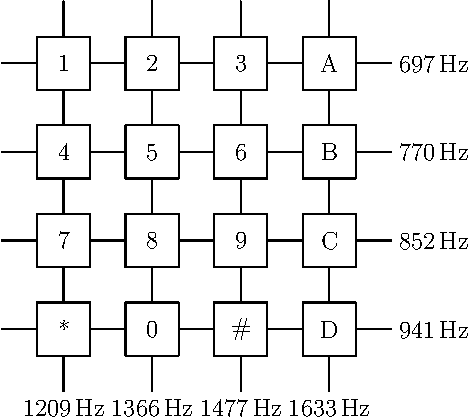
\includegraphics[height=.4\textheight]{pic/dtmf.pdf}
        \end{figure}
    \end{minipage}
\end{frame}


\begin{frame}[fragile]{\LaTeX{} Common Commands}
    \begin{exampleblock}{Commands}
        \centering
        \footnotesize
        \begin{tabular}{llll}
            \cmd{chapter} & \cmd{section} & \cmd{subsection} & \cmd{paragraph} \\
            chapter & section & sub-section & paragraph \\\hline
            \cmd{centering} & \cmd{emph} & \cmd{verb} & \cmd{url} \\
            center & emphasize & original & hyperlink \\\hline
            \cmd{footnote} & \cmd{item} & \cmd{caption} & \cmd{includegraphics} \\
            footnote & list item & caption & insert image \\\hline
            \cmd{label} & \cmd{cite} & \cmd{ref} \\
            label & citation & refer\\\hline
        \end{tabular}
    \end{exampleblock}
    \begin{exampleblock}{Environment}
        \centering
        \footnotesize
        \begin{tabular}{lll}
            \env{table} & \env{figure} & \env{equation}\\
            table & figure & formula \\\hline
            \env{itemize} & \env{enumerate} & \env{description}\\
            non-numbering item & numbering item & description \\\hline
        \end{tabular}
    \end{exampleblock}
\end{frame}

\begin{frame}[fragile]{\LaTeX{} Examples of environmental commands}
    \begin{minipage}{0.5\linewidth}
\begin{lstlisting}[language=TeX]
\begin{itemize}
  \item A \item B
  \item C
  \begin{itemize}
    \item C-1
  \end{itemize}
\end{itemize}
\end{lstlisting}
    \end{minipage}\hspace{1cm}
    \begin{minipage}{0.3\linewidth}
        \begin{itemize}
            \item A
            \item B
            \item C
            \begin{itemize}
                \item C-1
            \end{itemize}
        \end{itemize}
    \end{minipage}
    \medskip
    \pause
    \begin{minipage}{0.5\linewidth}
\begin{lstlisting}[language=TeX]
\begin{enumerate}
  \item A \item B
  \item C
  \begin{itemize}
    \item[n+e]
  \end{itemize}
\end{enumerate}
\end{lstlisting}
    \end{minipage}\hspace{1cm}
    \begin{minipage}{0.3\linewidth}
        \begin{enumerate}
            \item A
            \item B
            \item C
            \begin{itemize}
                \item[n+e]
            \end{itemize}
        \end{enumerate}
    \end{minipage}
\end{frame}

\begin{frame}[fragile]{\LaTeX{} Formulas}
    \begin{columns}
        \begin{column}{.55\textwidth}
\begin{lstlisting}[language=TeX]
$V = \frac{4}{3}\pi r^3$

\[
  V = \frac{4}{3}\pi r^3
\]

\begin{equation}
  \label{eq:vsphere}
  V = \frac{4}{3}\pi r^3
\end{equation}
\end{lstlisting}
        \end{column}
        \begin{column}{.4\textwidth}
            $V = \frac{4}{3}\pi r^3$
            \[
                V = \frac{4}{3}\pi r^3
            \]
            \begin{equation}
                \label{eq:vsphere}
                V = \frac{4}{3}\pi r^3
            \end{equation}
        \end{column}
    \end{columns}
    \begin{itemize}
        \item more information \href{https://ja.overleaf.com/learn/latex/Mathematical_expressions}{\color{purple}{here}}
    \end{itemize}
\end{frame}

\begin{frame}[fragile]
    \begin{columns}
        \column{.6\textwidth}
\begin{lstlisting}[language=TeX]
\begin{table}[htbp]
  \caption{numbers & meaning}
  \label{tab:number}
  \centering
  \begin{tabular}{cl}
    \toprule
    number & meaning \\
    \midrule
    1 & 4.0 \\
    2 & 3.7 \\
    \bottomrule
  \end{tabular}
\end{table}
\end{lstlisting}
        \column{.4\textwidth}
        \begin{table}[htpb]
            \centering
            \caption{numbers \& meaning}
            \label{tab:number}
            \begin{tabular}{cl}\toprule
                numbers & meaning \\\midrule
                1 & 4.0\\
                2 & 3.7\\\bottomrule
            \end{tabular}
        \end{table}
        \normalsize formula~(\ref{eq:vsphere}) at previous slide and Table~\ref{tab:number}。
    \end{columns}
\end{frame}

% --------------------------------------
\section{Project Timeline}
\begin{frame}
    \begin{itemize}
        \item January: Literature review
        \item February: Reproduce and evaluate Beamer themes
        \item March to April: Beautify Monash Beamer theme
        \item May: Thesis writing
    \end{itemize}
\end{frame}

% --------------------------------------
\section{References}

\begin{frame}[allowframebreaks]
    \bibliography{ref}
    \bibliographystyle{alpha}
\end{frame}

% --------------------------------------
\begin{frame}
    \begin{center}
        {\Huge\calligra Thanks!}
    \end{center}
\end{frame}

\end{document}